\documentclass{article}
\usepackage{tikz}
\usetikzlibrary{angles, quotes}
\usepackage{amssymb}
\usepackage{physics}
\usepackage{pgfplots}
\pgfplotsset{width=10cm,compat=1.9}
\usepgfplotslibrary{statistics}
\usepackage[left=2.54cm,right=2.54cm,top=2.54cm,bottom=2.54cm]{geometry}
\usepackage{tasks} %Paquete necesario para la producción de items horizontales para algunos ejercicios de tarea empleando el comando /begin{multicols}}{#}.../end{multicols} para ayudarnos a reducir las páginas
\usepackage{pdflscape} %comando que permite cambiar a orientación horizontal las hojas%
\usepackage{soul} %Paquete para permitir la compilación de acentos usando el comando {\hl{}}}\\
\sethlcolor{yellow(munsell)} %comando para definir el color para el subrayado usando el comando \hl
\usepackage[utf8]{inputenc}
\usepackage[spanish]{babel}
\usepackage{icomma}
\usepackage{ragged2e}		
\usepackage{siunitx}
\usepackage{url}
\usepackage[colorlinks=true, urlcolor=blue,  linkcolor=Cerulean, citecolor=green]{hyperref}
\usepackage{pdfpages}
\usepackage{blindtext} %Paquete que genera texto ficticio (dummy text) con el comando: \blindtext
\usepackage{cancel} %in the preamble gives you four different modes of striking through: \cancel{text to cancel} draws a diagonal line (slash) through its argument, \bcancel{text to cancel} uses the negative slope (a backslash), \xcancel{text to cancel} draws an X (actually \cancel plus \bcancel), \cancelto{〈value〉}{〈expression〉} draws a diagonal arrow through the 〈expression〉pointing to the 〈value〉 (math-mode only)
\usepackage{csquotes}
\usepackage{afterpage}
\usepackage{parskip} 
\usepackage{float}
\usepackage{enumitem}
%\usepackage{multicol}%Paquete que permite la creación aislada de columnas de texto. De esta forma se reduce la cantidad de páginas en nuestro documento
\usepackage{lipsum} %Paquete que genera texto de relleno al igual que \usepackage{blindtext}, se usa con el comando \lipsum[#-#] los #(hashtags) delimitan el número de páginas que deseamos ocupar del paquete lipsum para usarlos como relleno. 

% Definir el comando personalizado para la nota
\newcommand{\mynote}[1]{%
\begin{tikzpicture}[baseline=-0.75ex]
\node[draw, circle, fill=Apple Green!60, inner sep=2pt] (note) {\textbf{Nota:}};
\end{tikzpicture}%
\ \textit{#1}%
}

% Definición de comandos para variables con barra
\newcommand{\xbar}{\overline{x}}
\newcommand{\ybar}{\overline{y}}

\newenvironment{Figura}
{\par\medskip\noindent\minipage{\linewidth}}
{\endminipage\par\medskip}
\usepackage{caption}
\usepackage[
backend=biber,
sorting=none,
url=true
]{biblatex} %bibliografía
\addbibresource{biblio.bib}
% Establecer el espacio entre las entradas de la bibliografía
\setlength{\bibitemsep}{1\baselineskip} % Puedes ajustar el valor según tus preferencias
\usepackage{amsmath,amsthm,amssymb,amsfonts}
\usepackage{pifont} %Permite la compilación del comando \xmark: es el símbolo de la tachita
\usepackage{mathtools} %permite la compilación de símbolos para matrices
\usepackage{empheq} %Paquete que se relaciona con \usepackage[most]{tcolorbox} para la creación de cuadros/cajas de colores para delimitar los resultados matemáticos o líneas de texto usando la línea de comando: \begin{empheq}[box={\mymath[colback=orange(webcolor)!70,drop lifted shadow]}]{equation*} \end{empheq}
\usepackage[most]{tcolorbox} %Paquete que se relaciona con \usepackage{empheq} para la creación de cuadros/cajas de colores para delimitar los resultados matemáticos o líneas de texto
\renewcommand{\qedsymbol}{$\blacksquare$}
\usetikzlibrary{positioning,decorations.pathreplacing} %Paquete que permite la compilación de llaves para cuadros sinópticos (brace diagram) 
\usepackage{schemata} %The schemata package is designed just for these brace diagrams
\usepackage{booktabs}

\newcommand\AB[2]{\schema{\schemabox{#1}}{\schemabox{#2}}} %comando o paquete necesario para crear cuadros sinópticos

\newtcbox{\mymath}[1][]{%
nobeforeafter, math upper, tcbox raise base,
enhanced, colframe=blue!30!black,
colback=blue!30, boxrule=1pt,
#1} %Comando importante para encasillar los resultados matemáticos en cajas de diferentes colores, se relaciona con los paquetes \usepackage{empheq} y \usepackage[most]{tcolorbox} 

\newenvironment{sysmatrix}[1]
{\left(\begin{array}{@{}#1@{}}}
{\end{array}\right)}
\newcommand{\ro}[1]{%
\xrightarrow{\mathmakebox[\rowidth]{#1}}%
}
\newlength{\rowidth}% row operation width
\AtBeginDocument{\setlength{\rowidth}{3em}}  %Comando importante para laproducción de lineas de operaciones entre matrices, método de Gauss o Gauss Jordan se relaciona con \newenvironment{sysmatrix}

%formato para cambiar el horario a español
\usepackage[spanish]{datetime2}
\DTMsetdatestyle{spanish}

\renewcommand{\today}{\DTMdisplaydate{\the\year}{\the\month}{\the\day }{-1}}
%%%%%%%%%%%%%%%%%%%%%%%%%%%%%%%%%%%%%%%%%

\usepackage{datetime}
\newcommand{\mycurrenttime}{\xxivtime}

%%%%%%%%%%%%%%%%%%%%%%%%%%%%%%%%%%%%%%%%%%%%%%%%%%%%%%%%%%%%%%%%%%%%%%%%%%%%%%%%%%%%%%%%%%%%%%%%%%%%%%%%%%%%%%%%%%%%%%%%%%%%%%%%%%%%%%%%%%%%%%%%%


%%%%%%%%%%%%%Caja de color para el título%%%%%%%%%%%%%%%%%%%%%%%%%%%%%%%%%%%%%%%%%%%%%%%%%%%%%%

\definecolor{myframecolor}{RGB}{1, 45, 75} % Prussian Blue
\definecolor{myboxcolor}{RGB}{0, 107, 92} % Apple Green

\newtcolorbox{mybox}{
enhanced,
colback=myboxcolor!7, % Color de fondo del cuadro
colframe=myframecolor, % Color del marco del cuadro
arc=0pt,
boxrule=1pt,
borderline west={2mm}{-10mm}{myframecolor}, % Borde en el lado izquierdo
sharp corners=southwest,
width=\linewidth,
before=\par\vspace{\bigskipamount}, % Espacio antes del cuadro
after=\par\vspace{\bigskipamount} % Espacio después del cuadro
}

%%%%%%%%%%%%%%%%%%%%%%%%%%%%%%%%%%%%%%%%%%%%%%%%%%%%%%%%%Nueva caja%%%%%%%%%%%%%%%%%%%%%%%%%%%%%%%%%%%%%%%%%%%%%%%%%%%%%%%%%%%%%%%%%

\newtcolorbox{mybox2}{
enhanced,
colback=Apple Green!7, % Color de fondo del cuadro
colframe=Apple Green, % Color del marco del cuadro
arc=0pt,
boxrule=1pt,
borderline west={2mm}{-10mm}{Apple Green}, % Borde en el lado izquierdo
sharp corners=southwest,
width=\linewidth,
before=\par\vspace{\bigskipamount}, % Espacio antes del cuadro
after=\par\vspace{\bigskipamount} % Espacio después del cuadro
}


\newcommand{\euler}{e} %Comando para producir letra e de euler
\newenvironment{remark}{\par\vfill\footnotesize % Vertical white space above the remark and smaller font size
\begin{list}{}{
	\leftmargin=80pt % Indentation on the left
	\rightmargin=60pt}\item\ignorespaces % Indentation on the right
\makebox[-2.5pt]{\begin{tikzpicture}[overlay]
		\node[draw=Horizon!60,line width=2.5pt,circle,fill=Horizon!25,font=\sffamily\bfseries,inner sep=4pt,outer sep=0pt] at (-19pt,5pt){\textcolor{Horizon}{Nota}};\end{tikzpicture}} % Blue Nota in a circle
\advance\baselineskip -1pt}{\end{list}\vskip5pt} % Tighter line spacing and white space after remark
\usepackage{graphicx}

\usepackage{titling}

\input{colores.tex}

%%Producir signos de cita textual``Asignatura''

\newcommand{\xmark}{\ding{55}} %%%comando que genera la tachita

\newenvironment{MyColorPar}[1]{%
\leavevmode\color{#1}\ignorespaces%
}{%
}%

%%%%%%%%%%%%%%%%%%% Título de la tarea, Nombre de alumno

\title{ \textcolor{Sun}{\textbf{Tarea \textcolor{onyx}{\textbf{\#{4}}}: \textcolor{Cinnabar}{\textbf{Gran canónico y estadística cuántica}}}}}
\author{\emph{Julio Alfredo Ballinas García} $\boldsymbol{\mid}$ \textcolor{Tarawera}{\textbf{202107583}}}
\date{\today}

%%%%%%%%%%%%%%%%%%% Datos de la Materia

\usepackage{fancyhdr}
\fancypagestyle{plain}{%  the preset of fancyhdr 
\fancyhf{} % clear all header and footer fields
\fancyfoot[R]{
\includegraphics[width=2cm]{LogoFCFMBUAP (1).png}}
\fancyfoot[L]{{\bfseries{\thedate{}}} a las {\bfseries{\mycurrenttime{}}} horas{} (GMT-6, H. Puebla de Zaragoza, Pue)}
\fancyhead[L]{\textbf{Asignatura:} Mecánica Estadística}
\fancyhead[R]{\theauthor}
}
\makeatletter
\def\@maketitle{%
\newpage
\null%
\begin{center}%
\let \footnote \thanks
{\LARGE \@title \par}%
\vskip 1em%
%{\large \@date}%
\end{center}%
}
\makeatother

\usepackage{lipsum}  
\usepackage{cmbright}


%%%%%%%%%%%%%%%%%%%%%%%%%%%%%%%%%%%%%%%%%%%%%%%%%%%%%%%%%%%%%%%%%%%%%%%%%%%%%%%%%%%%%%%%%%%%%%%%%%%%%%%%%%%%%%%%%%%%%%%%%%%%%%%%%%%%%%%%%%%%%%%%%%%%%%%%%%%%%%%%%%%%%%%%%%%%%%%%%%%%%%%%%%%%%%%%%%%%%%

% Por si el color se llama "Apple Green" con espacio en colores.tex:
\colorlet{AppleGreen}{Apple Green}

% Caja AppleGreen con tono ajustable
\newenvironment{AGbox}[1][7]% 7 = tono por defecto (más grande => más claro)
{%
  \begin{tcolorbox}[
    enhanced, breakable,
    colframe=AppleGreen,
    colback=AppleGreen!#1,
    boxrule=1pt,
    borderline west={2mm}{-10mm}{AppleGreen},
    sharp corners=southwest,
    left=14pt,right=14pt,top=10pt,bottom=10pt,
     boxsep=6pt,
  ]%
}{%
  \end{tcolorbox}%
}


\begin{document}



\maketitle

%%%%%%%%%%%%%%%%%%% Datos del profesor, campus, aula e integrantes

\begin{mybox2}
\noindent
\begin{tabular}{@{}p{3.7cm}p{10.4cm}@{}}
\textbf{Profesor} & Dr. Jorge Velázquez Castro \\[3pt]
\textbf{Campus / Facultad} & \textcolor{prussianblue}{\textbf{C.U. BUAP}} / \textcolor{trueblue}{\textbf{FCFM}} \\[3pt]
\textbf{Edificio / Salón} & \textcolor{prussianblue}{\textbf{EMA4}} / \textcolor{trueblue}{\textbf{407}} \\[6pt]
\end{tabular}
\end{mybox2}
\vspace{1cm}


% Solo el índice en negro y en negritas
\hypersetup{linkcolor=black}   % (opcional: urlcolor=black, citecolor=black)
{\bfseries \tableofcontents}
\hypersetup{linkcolor=Cerulean} % regresamos a tu paleta

\vspace{0.5cm}
\begin{center}
\begin{tikzpicture}
	% Dibuja círculos rellenos en diferentes colores
	\fill[bittersweet] (0,0) circle (0.17cm);
	\fill[Apple Green] (0.6,0) circle (0.17cm);
	\fill[trueblue] (1.2,0) circle (0.17cm);
	\fill[Aguamarina] (1.8,0) circle (0.17cm);
	\fill[Sun] (2.4,0) circle (0.17cm);
	\fill[orange(colorwheel)] (3.0,0) circle (0.17cm);
	\fill[Pesto] (3.6,0) circle (0.17cm);
	\fill[blue-violet] (4.2,0) circle (0.17cm);
	\fill[ticklemepink] (4.8,0) circle (0.17cm);
	\fill[Gallery] (5.4,0) circle (0.17cm);
	\fill[Mantle] (6.0,0) circle (0.17cm);
	\fill[Nevada] (6.6,0) circle (0.17cm);
	\fill[onyx] (7.2,0) circle (0.17cm);
	% Agrega más círculos o modifica los colores según sea necesario
\end{tikzpicture}
\end{center}  \vspace{0.5cm}

\setlength{\columnsep}{2cm}
\section*{\textcolor{Tarawera}{\textbf{Lista de problemas y soluciones}}}
\addcontentsline{toc}{section}{Problemas: \textcolor{Tarawera}{\textbf{Gran canónico y estadística cuántica}}}

%=========================================================
%                      Problema 1
%=========================================================

\addcontentsline{toc}{subsection}{\textcolor{Apple Green}{\textbf{\underline{Problema 1}}}}

\begin{AGbox}[8]
\textcolor{Apple Green}{\textbf{\underline{Problema 1}}} \vspace{2mm}

Consider an adsorbent surface having N sites, each of which can adsorb one gas
molecule. This surface is in contact with an ideal gas with chemical potential $\mu$
(determined by the pressure $p$ and temperature $T$). Assuming that the adsorbed
molecule has energy $-\epsilon_{0}$ compared to one in a free state.

\begin{enumerate}
    \item Find the \textbf{grand canonical partition} \textcolor{Cinnabar}{\textbf{function}}

    \item Calculate the covering ratio $\theta$, i.e., the ratio of adsorbed molecules to
    adsorbing sites on the surface.
\end{enumerate}

\textbf{Note}: A useful relation is: \[(1 + x)^{N} = \sum_{N_1} \frac{N!}{N_1! (N - N_1)!} x^{N_1}\]
\end{AGbox} \vspace{0.5cm}

\textcolor{Tuscany}{\textbf{Solución:}}

Para empezar, \emph{identificamos el modelo físico} que describe el sistema.  
Tenemos una superficie con \hbox{$N$} sitios de adsorción, y cada sitio puede estar en uno de dos estados:

Los posibles estados de un sitio son:

\begin{itemize}
    \item[$\bullet$] Sitio vacío (sin molécula adsorbida)
    \item[$\bullet$] Sitio ocupado por \emph{una} molécula de gas
\end{itemize}


La superficie está en contacto con un \textcolor{Lochinvar}{\textbf{reservorio de partículas}} (el gas ideal) caracterizado por el \emph{potencial químico} \(\mu\) y la temperatura \(T\). Esto significa que el número de moléculas adsorbidas sobre la superficie puede fluctuar, por lo que el ensamble adecuado es el \textcolor{Cinnabar}{\textbf{gran canónico}}.  

Definimos como siempre
\begin{equation}
\begin{split}
\beta &\equiv \frac{1}{k_{B}T}
\end{split}\label{eq:def_beta_gran}
\end{equation}

Supongamos que el número de moléculas adsorbidas sobre la superficie es $N_{1}$. Entonces:

\begin{itemize}
    \item[$\bullet$] El número total de sitios es $N$
    \item[$\bullet$] El número de sitios ocupados es $N_{1}$
    \item[$\bullet$] El número de sitios vacíos es $N - N_{1}$
\end{itemize}


Por hipótesis del problema, \emph{cada molécula adsorbida} tiene energía \(\,-\epsilon_{0}\) (medida respecto al estado libre).  
Tomando la energía del sitio vacío como \(\,0\), la energía total de una configuración con \(N_{1}\) moléculas adsorbidas es
\begin{equation}
\begin{split}
E(N_{1}) &= -\,\epsilon_{0}\,N_{1}
\end{split}\label{eq:energia_N1}
\end{equation}

Además, para cada valor de \(N_{1}\), hay un número de configuraciones \emph{degeneradas}, dependiendo de en qué sitios se coloquen las moléculas. El número de formas de escoger \(N_{1}\) sitios ocupados entre \(N\) sitios totales es el coeficiente binomial
\begin{equation}
\begin{split}
g(N_{1}) &= \frac{N!}{N_{1}!\,(N-N_{1})!}
\end{split}\label{eq:degeneracion_N1}
\end{equation}

En el \textcolor{Tarawera}{\textbf{ensamble gran canónico}}, la gran función de partición se define como
\begin{equation}
\begin{split}
\Xi(\mu,T)
&= \sum_{N_{1}=0}^{N} g(N_{1})\,
\exp\!\big[-\beta\big(E(N_{1}) - \mu N_{1}\big)\big]
\end{split}\label{eq:Xi_def_general}
\end{equation}
donde el factor \(\exp\!\big[-\beta(E-\mu N_{1})\big]\) pesa simultáneamente energía y número de partículas adsorbidas.

%---------------------------------------------------------
% 1) Gran función de partición
%---------------------------------------------------------

Sustituimos ahora las expresiones \eqref{eq:energia_N1} y \eqref{eq:degeneracion_N1} en \eqref{eq:Xi_def_general}. Obtenemos
\begin{equation}
\begin{split}
\Xi(\mu,T)
&= \sum_{N_{1}=0}^{N}
\frac{N!}{N_{1}!\,(N-N_{1})!}\,
\exp\!\big[-\beta\big(-\epsilon_{0}N_{1} - \mu N_{1}\big)\big] \\[4pt]
&= \sum_{N_{1}=0}^{N}
\frac{N!}{N_{1}!\,(N-N_{1})!}\,
\exp\!\Big[\beta(\epsilon_{0} + \mu)N_{1}\Big]
\end{split}\label{eq:Xi_paso1}
\end{equation}

Es conveniente introducir el factor
\begin{equation}
\begin{split}
x &\equiv e^{\beta(\epsilon_{0}+\mu)}
\end{split}\label{eq:def_x}
\end{equation}
de modo que \(\exp\!\big[\beta(\epsilon_{0}+\mu)N_{1}\big] = x^{N_{1}}\). Entonces
\begin{equation}
\begin{split}
\Xi(\mu,T)
&= \sum_{N_{1}=0}^{N}
\frac{N!}{N_{1}!\,(N-N_{1})!}\, x^{N_{1}}
\end{split}\label{eq:Xi_paso2}
\end{equation}

Aquí es exactamente donde usamos la relación que el problema proporciona:
\[
(1+x)^{N} = \sum_{N_{1}=0}^{N} \frac{N!}{N_{1}!\,(N-N_{1})!} x^{N_{1}}
\]
Comparando con \eqref{eq:Xi_paso2}, vemos que la suma tiene la \emph{misma estructura} que el desarrollo binomial. Por lo tanto,
\begin{equation}
\boxed{
\Xi(\mu,T)
= \big(1 + e^{\beta(\epsilon_{0}+\mu)}\big)^{N}
}
\label{eq:Xi_final}
\end{equation}
Esta es la \textcolor{Cinnabar}{\textbf{gran función de partición}} del sistema de adsorción con \(N\) sitios independientes.

También se puede interpretar como
\begin{equation}
\begin{split}
\Xi(\mu,T)
&= \big[\Xi_{1}(\mu,T)\big]^{N}
\end{split}\label{eq:Xi_factorizada}
\end{equation}
donde \(\Xi_{1}\) es la gran función de partición de un \emph{solo sitio}:
\begin{equation}
\begin{split}
\Xi_{1}(\mu,T)
&= 1 + e^{\beta(\epsilon_{0}+\mu)}
\end{split}\label{eq:Xi1_final}
\end{equation}
confirmando la independencia entre sitios.

%---------------------------------------------------------
% 2) Cociente de cobertura θ
%---------------------------------------------------------

Ahora queremos calcular la \emph{razón de cobertura} \(\theta\), definida como
\begin{equation}
\begin{split}
\theta
&\equiv \frac{\text{número promedio de moléculas adsorbidas}}{\text{número de sitios}} \\[4pt]
&= \frac{\langle N_{1} \rangle}{N}
\end{split}\label{eq:def_theta}
\end{equation}

En el ensamble gran canónico, el número promedio de partículas adsorbidas se obtiene a partir de \(\Xi\). Es usual emplear la identidad
\begin{equation}
\begin{split}
\langle N_{1} \rangle
&= \pdv{\ln \Xi}{(\beta\mu)}
\end{split}\label{eq:N_prom_deriv}
\end{equation}
Esta expresión se deduce al derivar la definición de \(\Xi\) respecto a \(\beta\mu\) y reconocer que cada término trae consigo un factor \(N_{1}\).

A partir de \eqref{eq:Xi_final}, tenemos
\begin{equation}
\begin{split}
\ln \Xi(\mu,T)
&= N \ln\big(1 + e^{\beta(\epsilon_{0}+\mu)}\big)
\end{split}\label{eq:log_Xi}
\end{equation}

Tomamos ahora la derivada respecto de \(\beta\mu\). Observemos primero que
\begin{equation}
\begin{split}
\beta(\epsilon_{0}+\mu)
&= \beta\epsilon_{0} + \beta\mu
\end{split}\label{eq:beta_argumento}
\end{equation}
Si tratamos \(\beta\mu\) como la variable de derivación, \(\beta\epsilon_{0}\) es una constante. Derivando \eqref{eq:log_Xi}, obtenemos
\begin{equation}
\begin{split}
\pdv{\ln \Xi}{(\beta\mu)}
&= N\,
\frac{1}{1 + e^{\beta(\epsilon_{0}+\mu)}}\,
\pdv{}{(\beta\mu)}\Big[e^{\beta(\epsilon_{0}+\mu)}\Big] \\[4pt]
&= N\,
\frac{1}{1 + e^{\beta(\epsilon_{0}+\mu)}}\,
e^{\beta(\epsilon_{0}+\mu)} \\[4pt]
&= N\,
\frac{e^{\beta(\epsilon_{0}+\mu)}}{1 + e^{\beta(\epsilon_{0}+\mu)}}
\end{split}\label{eq:deriv_logXi}
\end{equation}
Usando \eqref{eq:N_prom_deriv}, concluimos que
\begin{equation}
\begin{split}
\langle N_{1} \rangle
&= N\,
\frac{e^{\beta(\epsilon_{0}+\mu)}}{1 + e^{\beta(\epsilon_{0}+\mu)}}
\end{split}\label{eq:N_promedio_final}
\end{equation}

Sustituimos este resultado en la definición de \(\theta\) en \eqref{eq:def_theta}:
\begin{equation}
\begin{split}
\theta
&= \frac{\langle N_{1} \rangle}{N} \\[4pt]
&= \frac{N\,\dfrac{e^{\beta(\epsilon_{0}+\mu)}}{1 + e^{\beta(\epsilon_{0}+\mu)}}}{N} \\[4pt]
&= \frac{e^{\beta(\epsilon_{0}+\mu)}}{1 + e^{\beta(\epsilon_{0}+\mu)}}
\end{split}\label{eq:theta_final}
\end{equation}

Podemos encerrar este resultado en un recuadro, pues es la expresión final buscada para la razón de cobertura:
\begin{equation}
\boxed{
\theta
= \frac{e^{\beta(\epsilon_{0}+\mu)}}{1 + e^{\beta(\epsilon_{0}+\mu)}}
}
\label{eq:theta_boxed}
\end{equation}

Es interesante notar que la forma de \(\theta\) en \eqref{eq:theta_boxed} es análoga a un \emph{factor de ocupación tipo Fermi–Dirac} para un nivel de energía \(-\epsilon_{0}\) en contacto con un reservorio de partículas con potencial químico \(\mu\). Aquí, la restricción de “un sitio, a lo más una partícula” hace que la estadística efectiva de ocupación adopte esta forma \textbf{sigmoide}.

En este contexto, la \textcolor{Lochinvar}{\textbf{cobertura}} \(\theta\) se interpreta como la \emph{fracción promedio de sitios ocupados} en la superficie:
\[
\theta = \frac{\langle N_{1} \rangle}{N}
\]
De modo que:
\begin{itemize}
    \item[$\bullet$] Si \(\theta \approx 0\), casi todos los sitios están vacíos
    \item[$\bullet$] Si \(\theta \approx 1\), la superficie está prácticamente saturada
\end{itemize}

La dependencia sigmoide de \(\theta\) con el potencial químico reducido \(\mu/\epsilon_{0}\) se muestra en la Fig.~\ref{fig:theta_vs_mu}. Para valores muy negativos de \(\mu\), la adsorción es desfavorable y la superficie permanece casi vacía. Conforme \(\mu\) aumenta, la probabilidad de ocupación crece y la cobertura pasa suavemente de \(0\) a \(1\).

\begin{figure}[H]
    \centering
    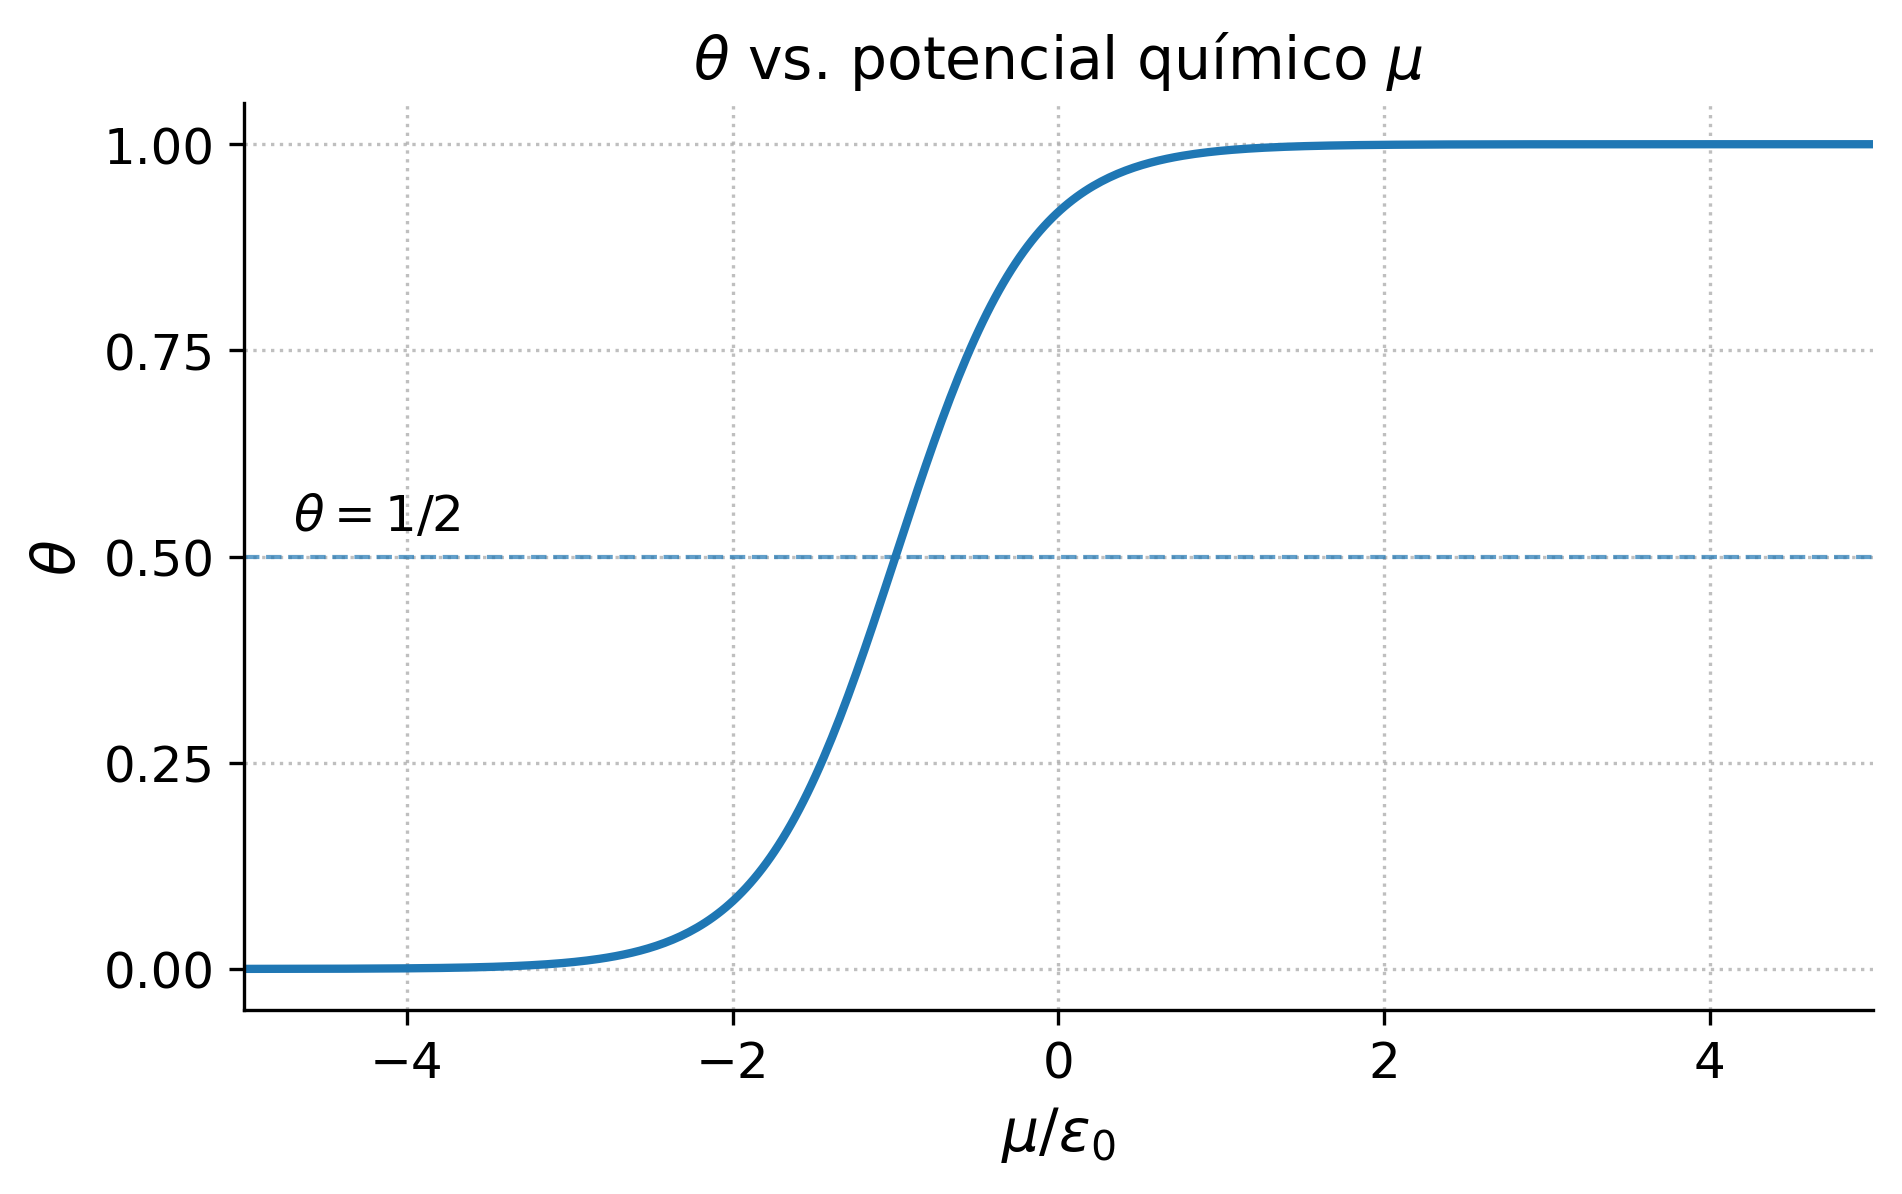
\includegraphics[width=0.7\textwidth]{theta_vs_mu.png}
    \caption{Cobertura $\theta$ en función del potencial químico reducido
    $\mu/\epsilon_{0}$ para el modelo de adsorción en una superficie con $N$
    sitios independientes. La curva sigmoide refleja la ocupación promedio de
    cada sitio en el ensamble gran canónico.}
    \label{fig:theta_vs_mu}
\end{figure}

En la Fig.~\ref{fig:theta_vs_mu_multiT} se compara el comportamiento de la cobertura para distintas temperaturas. A temperaturas bajas, la transición entre la superficie casi vacía y la superficie casi saturada es más brusca; al aumentar \(T\), las fluctuaciones térmicas suavizan la curva y la región de transición se ensancha.

\begin{figure}[H]
    \centering
    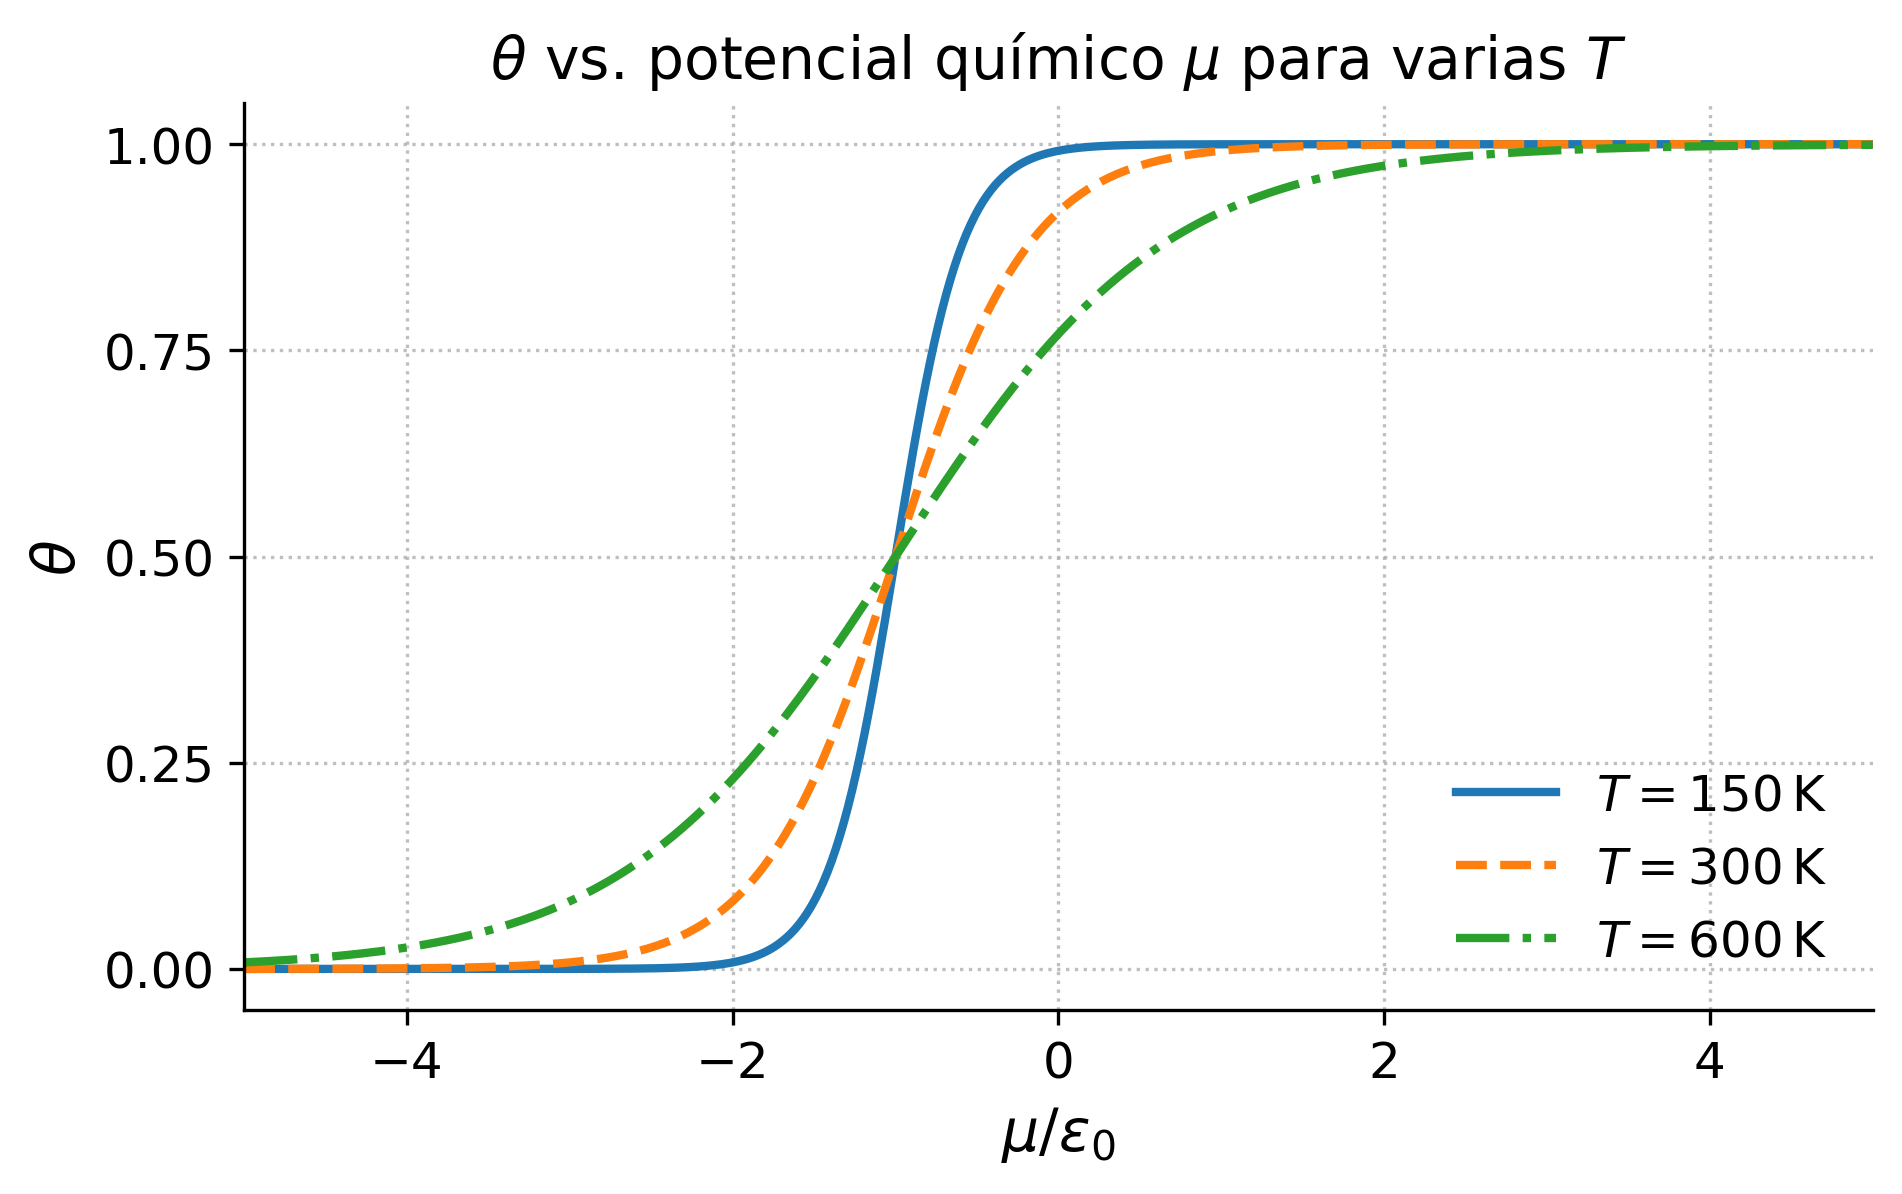
\includegraphics[width=0.7\textwidth]{theta_vs_mu_multiT.png}
    \caption{Cobertura $\theta$ en función del potencial químico reducido
    $\mu/\epsilon_{0}$ para distintas temperaturas $T$. Al aumentar la
    temperatura, la transición entre la superficie casi vacía
    ($\theta \approx 0$) y casi completamente cubierta ($\theta \approx 1$)
    se hace más suave debido al incremento de las fluctuaciones térmicas.}
    \label{fig:theta_vs_mu_multiT}
\end{figure}

Se puede usar la siguiente \textcolor{Apple Green}{\textbf{minitablita}} para esclarecer de manera visual los parámetros relevantes del modelo, 

\begin{table}[H]
    \centering
    \renewcommand{\arraystretch}{1.2}
    \begin{tabular}{ll}
        \colorbox{Tarawera}{\textcolor{Gallery}{\(\theta\)}} &
        Fracción promedio de sitios ocupados, \(\theta = \langle N_{1} \rangle / N\) \\[4pt]
        \colorbox{Apple Green}{\textcolor{Gallery}{\(\mu\)}} &
        Potencial químico del gas en el reservorio; controla cuántas moléculas tienden a adsorberse \\[4pt]
        \colorbox{Cinnabar}{\textcolor{Gallery}{\(\epsilon_{0}\)}} &
        Módulo de la energía de adsorción por molécula (la energía del estado adsorbido es \(-\epsilon_{0}\)) \\[4pt]
        \colorbox{Horizon}{\textcolor{Gallery}{\(T\)}} &
        Temperatura del sistema; al aumentar \(T\) la curva de $\theta(\mu)$ se vuelve más suave \\[4pt]
        \colorbox{Nevada}{\textcolor{Gallery}{\(N\)}} &
        Número total de sitios de adsorción disponibles en la superficie
    \end{tabular}
    \caption{Parámetros principales del modelo de adsorción en una superficie con sitios independientes.}
    \label{tab:parametros_adsorcion}
\end{table}



\vspace{0.6cm}

%=========================================================
%                      Problema 2
%=========================================================

\addcontentsline{toc}{subsection}{\textcolor{Apple Green}{\textbf{\underline{Problema 2}}}}
\begin{AGbox}[8]
\textcolor{Apple Green}{\textbf{\underline{Problema 2}}} \vspace{2mm}

Considere un sistema de dos átomos, cada uno de ellos sólo tiene 3 posibles
estados con energías \textcolor{Tarawera}{$\boldsymbol{0}$}, \textcolor{vividviolet}{$\boldsymbol{\epsilon}$} y \textcolor{orange(colorwheel)}{$\boldsymbol{2\epsilon}$}. El sistema está a temperatura $T$. Escribe la
\textcolor{Cinnabar}{\textbf{función de partición}} para el sistema si las partículas obedecen:

\begin{enumerate}
    \item La estadística de \textcolor{Lochinvar}{\textbf{Fermi-Dirac}} (son fermiones)

    \item La estadística de \textcolor{orange(colorwheel)}{\textbf{Bose-Einstein}} (son bosones)
\end{enumerate}
\end{AGbox} \vspace{0.5cm}

\textcolor{Tuscany}{\textbf{Solución:}}

En este problema tenemos un sistema muy pequeño: sólo hay \emph{dos átomos} y cada uno
puede ocupar \underline{tres niveles de energía} diferentes. Los niveles
de energía de una sola partícula son
\begin{equation}
\begin{split}
\varepsilon_{0} &= 0, \qquad
\varepsilon_{1} = \epsilon, \qquad
\varepsilon_{2} = 2\epsilon
\end{split}\label{eq:niveles_una_particula}
\end{equation}
El sistema está en equilibrio térmico a temperatura \(T\). Como el número de partículas
no cambia, trabajamos con el \textcolor{Tarawera}{\textbf{ensamble canónico}}, y la cantidad que debemos
construir es la \textcolor{Cinnabar}{\textbf{función de partición canónica}} del sistema de dos partículas:
\begin{equation}
\begin{split}
Z(T)
&= \sum_{\text{estados cuánticos }} e^{-\beta E}
\end{split}\label{eq:def_Z_generica}
\end{equation}
donde
\(\beta \equiv 1/(k_{B}T)\) y la suma recorre todos los \emph{estados de dos partículas} permitidos
por la estadística cuántica correspondiente.

La diferencia entre Fermi–Dirac y Bose–Einstein aparece en
\textcolor{Lochinvar}{\emph{cómo contamos}} los estados:
\begin{itemize}
    \item[$\bullet$] Para \textcolor{Lochinvar}{fermiones} (Fermi–Dirac): no pueden haber dos partículas en el mismo nivel
    de energía (\emph{principio de exclusión de Pauli}).
    \item[$\bullet$] Para \textcolor{orange(colorwheel)}{bosones} (Bose–Einstein): sí se permite que las dos partículas estén
    en el mismo nivel de energía.
\end{itemize}

Vamos a analizar cada caso por separado.

%---------------------------------------------------------
% 1) Fermiones (Fermi-Dirac)
%---------------------------------------------------------
\subsubsection*{\textcolor{Lochinvar}{Estadística de Fermi–Dirac (fermiones)}}

Suponemos que los dos átomos son fermiones \emph{idénticos} y que cada nivel de
energía de \eqref{eq:niveles_una_particula} es \emph{no degenerado}.  
El principio de exclusión nos dice que \textbf{sólo podemos ocupar niveles distintos}.

Con dos fermiones y tres niveles disponibles, los posibles conjuntos de ocupación son:
\begin{itemize}
    \item[$\bullet$] Un fermión en \(0\) y otro en \(\epsilon\)
    \item[$\bullet$] Un fermión en \(0\) y otro en \(2\epsilon\)
    \item[$\bullet$] Un fermión en \(\epsilon\) y otro en \(2\epsilon\)
\end{itemize}
(En todos los casos, el orden “quién está dónde” no importa, porque las partículas
son indistinguibles.)

A partir de \eqref{eq:niveles_una_particula}, las energías totales de estos
\emph{estados de dos partículas} son:
\begin{equation}
\begin{split}
E_{(0,\epsilon)} &= 0 + \epsilon = \epsilon \\[4pt]
E_{(0,2\epsilon)} &= 0 + 2\epsilon = 2\epsilon \\[4pt]
E_{(\epsilon,2\epsilon)} &= \epsilon + 2\epsilon = 3\epsilon
\end{split}\label{eq:energias_FD}
\end{equation}

Cada una de estas configuraciones tiene degeneración \(1\) (no hay más de un estado
simétrico/antisimétrico distinto, dado que los niveles de una sola partícula no
están degenerados). Por lo tanto, la función de partición del sistema fermiónico es
\begin{equation}
\begin{split}
Z_{\text{FD}}(T)
&= e^{-\beta E_{(0,\epsilon)}} + e^{-\beta E_{(0,2\epsilon)}} + e^{-\beta E_{(\epsilon,2\epsilon)}} \\[4pt]
&= e^{-\beta \epsilon}
   + e^{-\beta 2\epsilon}
   + e^{-\beta 3\epsilon}
\end{split}\label{eq:Z_FD_paso}
\end{equation}

En forma compacta, podemos encerrar el resultado en un recuadro:
\begin{equation}
\boxed{
Z_{\text{FD}}(T)
= e^{-\beta \epsilon}
  + e^{-\beta 2\epsilon}
  + e^{-\beta 3\epsilon}
}
\label{eq:Z_FD_final}
\end{equation}

%---------------------------------------------------------
% 2) Bosones (Bose-Einstein)
%---------------------------------------------------------
\subsubsection*{\textcolor{orange(colorwheel)}{Estadística de Bose–Einstein (bosones)}}

Ahora los dos átomos son bosones indistinguibles.  
En este caso, \emph{sí} podemos colocar las dos partículas en el mismo nivel de
energía. Conviene describir cada estado de dos partículas mediante los números de
ocupación \((n_{0},n_{1},n_{2})\), donde \(n_{j}\) indica cuántas partículas hay en el
nivel \(\varepsilon_{j}\) de \eqref{eq:niveles_una_particula}. Como sólo hay dos
partículas, estos números deben satisfacer:
\begin{equation}
\begin{split}
n_{0} + n_{1} + n_{2} = 2, \qquad
n_{0},n_{1},n_{2} \in \mathbb{N}_{0}
\end{split}\label{eq:cond_n_occup}
\end{equation}

Las posibles combinaciones \((n_{0},n_{1},n_{2})\) que cumplen \eqref{eq:cond_n_occup}
son:
\begin{itemize}
    \item[$\bullet$] \((2,0,0)\): dos bosones en el nivel de energía \(0\)
    \item[$\bullet$] \((0,2,0)\): dos bosones en el nivel de energía \(\epsilon\)
    \item[$\bullet$] \((0,0,2)\): dos bosones en el nivel de energía \(2\epsilon\)
    \item[$\bullet$] \((1,1,0)\): uno en \(0\) y uno en \(\epsilon\)
    \item[$\bullet$] \((1,0,1)\): uno en \(0\) y uno en \(2\epsilon\)
    \item[$\bullet$] \((0,1,1)\): uno en \(\epsilon\) y uno en \(2\epsilon\)
\end{itemize}

La energía de un estado caracterizado por \((n_{0},n_{1},n_{2})\) se obtiene sumando
las energías de las partículas:
\begin{equation}
\begin{split}
E(n_{0},n_{1},n_{2})
&= n_{0}\,\varepsilon_{0} + n_{1}\,\varepsilon_{1} + n_{2}\,\varepsilon_{2} \\[4pt]
&= n_{0}\cdot 0 + n_{1}\,\epsilon + n_{2}\,(2\epsilon)
\end{split}\label{eq:E_n0n1n2_general}
\end{equation}

Aplicando \eqref{eq:E_n0n1n2_general} a cada tripleta de ocupación, obtenemos:
\begin{equation}
\begin{split}
(2,0,0):\quad &E = 0 \\[4pt]
(0,2,0):\quad &E = 2\epsilon \\[4pt]
(0,0,2):\quad &E = 4\epsilon \\[4pt]
(1,1,0):\quad &E = \epsilon \\[4pt]
(1,0,1):\quad &E = 2\epsilon \\[4pt]
(0,1,1):\quad &E = 3\epsilon
\end{split}\label{eq:E_Bose_lista}
\end{equation}

Cada patrón de ocupación \((n_{0},n_{1},n_{2})\) corresponde, en este modelo simple
(sin degeneraciones adicionales), a un \emph{único} estado de dos bosones simétrico,
por lo que todos tienen degeneración \(1\). La función de partición se construye
sumando \(e^{-\beta E}\) sobre todos ellos:
\begin{equation}
\begin{split}
Z_{\text{BE}}(T)
&= e^{-\beta\cdot 0}
 + e^{-\beta\epsilon}
 + e^{-\beta 2\epsilon}
 + e^{-\beta 2\epsilon}
 + e^{-\beta 3\epsilon}
 + e^{-\beta 4\epsilon}
\end{split}\label{eq:Z_BE_paso1}
\end{equation}

Es útil agrupar términos con la misma energía. A partir de \eqref{eq:E_Bose_lista},
vemos que:
\begin{itemize}
    \item[$\bullet$] \(E=0\): una vez  
    \item[$\bullet$] \(E=\epsilon\): una vez  
    \item[$\bullet$] \(E=2\epsilon\): dos veces  
    \item[$\bullet$] \(E=3\epsilon\): una vez  
    \item[$\bullet$] \(E=4\epsilon\): una vez
\end{itemize}
Por ello, \eqref{eq:Z_BE_paso1} puede escribirse como
\begin{equation}
\begin{split}
Z_{\text{BE}}(T)
&= 1
 + e^{-\beta\epsilon}
 + 2e^{-\beta 2\epsilon}
 + e^{-\beta 3\epsilon}
 + e^{-\beta 4\epsilon}
\end{split}\label{eq:Z_BE_paso2}
\end{equation}

Finalmente, encerramos el resultado en un recuadro:
\begin{equation}
\boxed{
Z_{\text{BE}}(T)
= 1
 + e^{-\beta\epsilon}
 + 2e^{-\beta 2\epsilon}
 + e^{-\beta 3\epsilon}
 + e^{-\beta 4\epsilon}
}
\label{eq:Z_BE_final}
\end{equation}

Con \eqref{eq:Z_FD_final} y \eqref{eq:Z_BE_final} hemos obtenido la
\textcolor{Cinnabar}{\textbf{función de partición}} del sistema de dos partículas para los dos casos
pedidos: fermiones (Fermi–Dirac) y bosones (Bose–Einstein), respetando las reglas
de ocupación cuántica en cada caso.


\vspace{0.6cm}

%=========================================================
%                      Problema 3
%=========================================================

\addcontentsline{toc}{subsection}{\textcolor{Apple Green}{\textbf{\underline{Problema 3}}}}
\begin{AGbox}[8]
\textcolor{Apple Green}{\textbf{\underline{Problema 3}}} \vspace{2mm}

Considera un sistema clásico de moléculas diatómicas no interactuantes en una
caja de volumen $V$ a temperatura $T$ y potencial químico $\mu$. La hamiltoniana
de una sola molécula es

\[
H(r_{1}, r_{2}, p_{1}, p_{2}) = \frac{1}{2m}(p_{1}^{2} + p_{2}^{2}) + \frac{1}{2} K |r_{1} - r_{2}|^{2}
\]

\begin{itemize}
    \item[$\bullet$] Calcula la gran  \textcolor{Cinnabar}{\textbf{función de partición}}

    \item[$\bullet$] Calcula $\langle r_{12}^{2} \rangle$ como función de $T$ y $\mu$.
\end{itemize}
\end{AGbox} \vspace{0.5cm}

\textcolor{Tuscany}{\textbf{Solución:}}

En este problema tenemos un gas clásico de \emph{moléculas diatómicas} no
interactuantes en una caja de volumen \(V\), a temperatura \(T\) y en contacto con
un reservorio de partículas con potencial químico \(\mu\).  
Por tanto, el ensamble adecuado es el \textcolor{Tarawera}{\textbf{gran canónico}}.

Cada molécula está formada por dos átomos de masa \(m\). Las coordenadas de los
átomos son \(\vec r_{1}\) y \(\vec r_{2}\), y sus momentos canónicos \(\vec p_{1}\) y
\(\vec p_{2}\). La hamiltoniana de una sola molécula está dada por
\begin{equation}
\begin{split}
H(\vec r_{1},\vec r_{2},\vec p_{1},\vec p_{2})
&= \frac{1}{2m}\big(\vec p_{1}^{\,2} + \vec p_{2}^{\,2}\big)
   + \frac{1}{2}K\,|\vec r_{1} - \vec r_{2}|^{2}
\end{split}\label{eq:H_molecula_original}
\end{equation}
el primer término corresponde a la energía cinética de los dos átomos
y el segundo a una \emph{interacción armónica} entre ellos, con constante elástica \(K\).

Como siempre, definimos
\begin{equation}
\begin{split}
\beta &\equiv \frac{1}{k_{B}T}
\end{split}\label{eq:def_beta_prob3}
\end{equation}

%---------------------------------------------------------
% 1) Transformación a coordenadas de centro de masa y relativas
%---------------------------------------------------------

Es conveniente separar el movimiento de \emph{centro de masa} y el movimiento
\emph{relativo} dentro de la molécula. Definimos:
\begin{equation}
\begin{split}
\vec R &= \frac{\vec r_{1} + \vec r_{2}}{2}
\qquad\text{(centro de masa)}\\[4pt]
\vec r &= \vec r_{1} - \vec r_{2}
\qquad\text{(coordenada relativa)}
\end{split}\label{eq:def_R_r}
\end{equation}
y los momentos conjugados
\begin{equation}
\begin{split}
\vec P &= \vec p_{1} + \vec p_{2}
\qquad\text{(momento total)}\\[4pt]
\vec p &= \frac{\vec p_{1} - \vec p_{2}}{2}
\qquad\text{(momento relativo)}
\end{split}\label{eq:def_P_p}
\end{equation}

Esta transformación es lineal y canónica; en particular, el jacobiano es \(1\), de
modo que
\[
\dd[3]{r_{1}}\dd[3]{r_{2}}\,\dd[3]{p_{1}}\dd[3]{p_{2}}
= \dd[3]{R}\dd[3]{r}\,\dd[3]{P}\dd[3]{p}
\]

Sustituyendo \eqref{eq:def_P_p} en la parte cinética de
\eqref{eq:H_molecula_original}:
\begin{equation}
\begin{split}
\vec p_{1}^{\,2} + \vec p_{2}^{\,2}
&= \left(\frac{\vec P}{2} + \vec p\right)^{2}
 + \left(\frac{\vec P}{2} - \vec p\right)^{2} \\[4pt]
&= \frac{\vec P^{2}}{4} + 2\vec p^{\,2}
\end{split}\label{eq:p1p2_en_Pp}
\end{equation}
Por tanto,
\begin{equation}
\begin{split}
H
&= \frac{1}{2m}\left(\frac{\vec P^{2}}{4} + 2\vec p^{\,2}\right)
   + \frac{1}{2}K\,\vec r^{2} \\[4pt]
&= \frac{\vec P^{2}}{4m} + \frac{\vec p^{\,2}}{m}
   + \frac{1}{2}K\,\vec r^{\,2}
\end{split}\label{eq:H_en_RrPp}
\end{equation}

Vemos que la energía se \emph{factoriza} en una parte de \(\vec R,\vec P\) (movimiento
del centro de masa) y otra de \(\vec r,\vec p\) (movimiento interno de la molécula).

%---------------------------------------------------------
% 2) Función de partición canónica de una molécula
%---------------------------------------------------------

La función de partición canónica de \emph{una sola molécula} se define como
\begin{equation}
\begin{split}
Q_{1}(T,V)
&= \frac{1}{h^{6}}
\int \dd[3]{r_{1}}\dd[3]{r_{2}}\dd[3]{p_{1}}\dd[3]{p_{2}}\,
e^{-\beta H(\vec r_{1},\vec r_{2},\vec p_{1},\vec p_{2})}
\end{split}\label{eq:Q1_def_original}
\end{equation}
Usando la transformación \eqref{eq:def_R_r}–\eqref{eq:def_P_p} y la forma de la
hamiltoniana en \eqref{eq:H_en_RrPp}, esto se convierte en
\begin{equation}
\begin{split}
Q_{1}(T,V)
&= \frac{1}{h^{6}}\,
\int \dd[3]{R}\dd[3]{r}\dd[3]{P}\dd[3]{p}\,
\exp\!\left[-\beta\left(
\frac{\vec P^{2}}{4m} + \frac{\vec p^{\,2}}{m}
+ \frac{1}{2}K\,\vec r^{\,2}
\right)\right]
\end{split}\label{eq:Q1_en_RrPp}
\end{equation}

El integrando se separa en un producto de términos que dependen
de variables distintas. Esto nos permite factorizar la integral:
\begin{equation}
\begin{split}
Q_{1}(T,V)
&= \frac{1}{h^{6}}
\left[\int \dd[3]{R}\dd[3]{P}\,
e^{-\beta \vec P^{2}/(4m)}\right]
\left[\int \dd[3]{r}\dd[3]{p}\,
e^{-\beta\left(\vec p^{\,2}/m + \frac{1}{2}K\vec r^{\,2}\right)}\right]
\end{split}\label{eq:Q1_factorizada}
\end{equation}

Llamemos:
\begin{equation}
\begin{split}
Q_{\text{trans}}
&\equiv \frac{1}{h^{3}}
\int \dd[3]{R}\dd[3]{P}\,
e^{-\beta \vec P^{2}/(4m)} \\[4pt]
Q_{\text{int}}
&\equiv \frac{1}{h^{3}}
\int \dd[3]{r}\dd[3]{p}\,
e^{-\beta\left(\vec p^{\,2}/m + \frac{1}{2}K\vec r^{\,2}\right)}
\end{split}\label{eq:Qtrans_Qint_def}
\end{equation}
de modo que
\begin{equation}
\begin{split}
Q_{1}(T,V)
&= Q_{\text{trans}}\,Q_{\text{int}}
\end{split}\label{eq:Q1_Qtrans_Qint}
\end{equation}

\emph{Parte traslacional:} la integral en \(\vec R\) simplemente produce el volumen:
\begin{equation}
\begin{split}
\int \dd[3]{R} &= V
\end{split}\label{eq:int_R}
\end{equation}
y la integral gaussiana en \(\vec P\) es
\begin{equation}
\begin{split}
\int \dd[3]{P}\,e^{-\beta \vec P^{2}/(4m)}
&= \left(\frac{4\pi m}{\beta}\right)^{3/2}
\end{split}\label{eq:int_P}
\end{equation}
Así,
\begin{equation}
\begin{split}
Q_{\text{trans}}
&= \frac{1}{h^{3}}\,V\left(\frac{4\pi m}{\beta}\right)^{3/2}
\end{split}\label{eq:Qtrans_final}
\end{equation}

\emph{Parte interna:} tenemos un oscilador armónico en 3D en la coordenada \(\vec r\)
y un término cinético en \(\vec p\). Las integrales gaussianas son:
\begin{equation}
\begin{split}
\int \dd[3]{p}\,e^{-\beta \vec p^{\,2}/m}
&= \left(\frac{\pi m}{\beta}\right)^{3/2} \\[4pt]
\int \dd[3]{r}\,e^{-\beta K\vec r^{\,2}/2}
&= \left(\frac{2\pi}{\beta K}\right)^{3/2}
\end{split}\label{eq:int_p_r}
\end{equation}
por lo tanto,
\begin{equation}
\begin{split}
Q_{\text{int}}
&= \frac{1}{h^{3}}
\left(\frac{\pi m}{\beta}\right)^{3/2}
\left(\frac{2\pi}{\beta K}\right)^{3/2}
\end{split}\label{eq:Qint_final}
\end{equation}

Multiplicando \eqref{eq:Qtrans_final} y \eqref{eq:Qint_final} en
\eqref{eq:Q1_Qtrans_Qint}, obtenemos
\begin{equation}
\begin{split}
Q_{1}(T,V)
&= \frac{V}{h^{6}}
\left(\frac{4\pi m}{\beta}\right)^{3/2}
\left(\frac{\pi m}{\beta}\right)^{3/2}
\left(\frac{2\pi}{\beta K}\right)^{3/2}
\end{split}\label{eq:Q1_paso}
\end{equation}

Se puede simplificar observando que
\[
\left(\frac{4\pi m}{\beta}\right)^{3/2}
\left(\frac{\pi m}{\beta}\right)^{3/2}
= \left(\frac{4\pi^{2}m^{2}}{\beta^{2}}\right)^{3/2}
= 8\,\frac{\pi^{3}m^{3}}{\beta^{3}}
\]
y
\[
\left(\frac{2\pi}{\beta K}\right)^{3/2}
= \frac{(2\pi)^{3/2}}{\beta^{3/2}K^{3/2}}
\]
por lo que
\begin{equation}
\begin{split}
Q_{1}(T,V)
&= \frac{V}{h^{6}}\,
8\,\frac{\pi^{3}m^{3}}{\beta^{3}}\,
\frac{(2\pi)^{3/2}}{\beta^{3/2}K^{3/2}} \\[4pt]
&= \frac{V}{h^{6}}\,
16\sqrt{2}\,\pi^{9/2}\,\frac{m^{3}}{K^{3/2}}\,\beta^{-9/2}
\end{split}\label{eq:Q1_beta}
\end{equation}

Recordando que \(\beta^{-1}=k_{B}T\), podemos escribir
\begin{equation}
\boxed{
Q_{1}(T,V)
= \frac{16\sqrt{2}\,\pi^{9/2}}{h^{6}}
\,\frac{m^{3}}{K^{3/2}}\,
V\,(k_{B}T)^{9/2}
}
\label{eq:Q1_final}
\end{equation}
Esta es la \textcolor{Cinnabar}{\textbf{función de partición canónica}} para una molécula diatómica en
este potencial armónico interno.

%---------------------------------------------------------
% 3) Gran función de partición
%---------------------------------------------------------

Para un gas clásico ideal de moléculas indistinguibles en el ensamble gran
canónico, la \textcolor{Cinnabar}{\textbf{gran función de partición}} es
\begin{equation}
\begin{split}
\Xi(\mu,T,V)
&= \sum_{N=0}^{\infty}
\frac{1}{N!}\big[z\,Q_{1}(T,V)\big]^{N}
\end{split}\label{eq:Xi_def_prob3}
\end{equation}
donde
\begin{equation}
\begin{split}
z &\equiv e^{\beta\mu}
\end{split}\label{eq:def_z_prob3}
\end{equation}
es la \emph{actividad} del gas.

La suma en \eqref{eq:Xi_def_prob3} es el desarrollo de la exponencial:
\begin{equation}
\begin{split}
\Xi(\mu,T,V)
&= \exp\!\big[z\,Q_{1}(T,V)\big]
\end{split}\label{eq:Xi_exp_paso}
\end{equation}

Sustituyendo \eqref{eq:Q1_final}:
\begin{equation}
\boxed{
\Xi(\mu,T,V)
= \exp\!\left[
e^{\beta\mu}\,
\frac{16\sqrt{2}\,\pi^{9/2}}{h^{6}}
\,\frac{m^{3}}{K^{3/2}}\,
V\,(k_{B}T)^{9/2}
\right]
}
\label{eq:Xi_final_prob3}
\end{equation}

%---------------------------------------------------------
% 4) Cálculo de \langle r_{12}^{2} \rangle
%---------------------------------------------------------

La cantidad \(r_{12}^{2}\) se refiere al cuadrado de la distancia relativa entre
los dos átomos de una molécula:
\[
r_{12}^{2} = |\vec r_{1} - \vec r_{2}|^{2} = \vec r^{\,2}
\]
Es decir, es simplemente el módulo al cuadrado de la coordenada relativa \(\vec r\).

Debido a que el potencial interno es armónico,
\begin{equation}
\begin{split}
U_{\text{int}}(\vec r)
&= \frac{1}{2}K\,\vec r^{\,2}
= \frac{1}{2}K(x^{2}+y^{2}+z^{2})
\end{split}\label{eq:U_int_armonico}
\end{equation}
cada coordenada \(x\), \(y\), \(z\) contribuye con un término cuadrático independiente.
Por el \textcolor{Lochinvar}{\textbf{teorema de equipartición}}, a temperatura \(T\),
cada grado de libertad cuadrático aporta una energía promedio
\(\frac{1}{2}k_{B}T\). En el potencial \eqref{eq:U_int_armonico} hay tres términos
cuadráticos:
\begin{equation}
\begin{split}
\frac{1}{2}Kx^{2},\quad
\frac{1}{2}Ky^{2},\quad
\frac{1}{2}Kz^{2}
\end{split}\label{eq:terminos_cuadraticos}
\end{equation}

Por lo tanto, la energía potencial promedio es
\begin{equation}
\begin{split}
\left\langle U_{\text{int}}\right\rangle
&= \frac{3}{2}k_{B}T
\end{split}\label{eq:U_int_promedio}
\end{equation}
pero también
\begin{equation}
\begin{split}
\left\langle U_{\text{int}}\right\rangle
&= \frac{1}{2}K\,\left\langle \vec r^{\,2}\right\rangle
= \frac{1}{2}K\,\left\langle r_{12}^{2}\right\rangle_{\text{1 mol}}
\end{split}\label{eq:U_int_en_r2}
\end{equation}

Igualando \eqref{eq:U_int_promedio} y \eqref{eq:U_int_en_r2}:
\begin{equation}
\begin{split}
\frac{1}{2}K\,\left\langle r_{12}^{2}\right\rangle_{\text{1 mol}}
&= \frac{3}{2}k_{B}T
\end{split}\label{eq:igualando_ener}
\end{equation}
de donde se obtiene
\begin{equation}
\boxed{
\left\langle r_{12}^{2}\right\rangle_{\text{1 mol}}
= \frac{3k_{B}T}{K}
}
\label{eq:r12_prom_una_molecula}
\end{equation}

Este resultado es la \emph{distancia cuadrática promedio} entre los dos átomos
de una molécula individual, y depende sólo de \(T\) y de \(K\), \underline{no}
del potencial químico \(\mu\). Esto refleja que la distribución interna de la
molécula armónica está fijada por la temperatura, independientemente de cuántas
moléculas haya en el sistema.

Si quisiéramos el promedio de la \emph{suma} sobre todas las moléculas en el
ensamble gran canónico,
\[
\left\langle \sum_{j=1}^{N} r_{12,j}^{2} \right\rangle
\]
entonces éste sería
\begin{equation}
\begin{split}
\left\langle \sum_{j=1}^{N} r_{12,j}^{2} \right\rangle
&= \left\langle N \right\rangle\,
\left\langle r_{12}^{2}\right\rangle_{\text{1 mol}} \\[4pt]
&= \left\langle N \right\rangle\,
\frac{3k_{B}T}{K}
\end{split}\label{eq:sum_r2_total}
\end{equation}
y aquí sí aparece \(\mu\) a través de
\(\left\langle N \right\rangle = z\,Q_{1}(T,V) = e^{\beta\mu}Q_{1}(T,V)\).  

De cualquier forma, la expresión fundamental para la \emph{distancia cuadrática
promedio} de una molécula es la dada en \eqref{eq:r12_prom_una_molecula}.




\end{document}
